\begin{figure}[h]
	\centering
	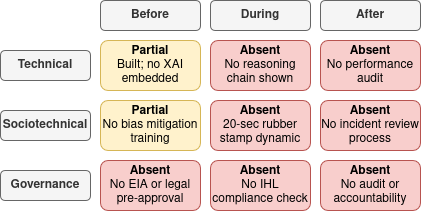
\includegraphics[width=0.8\textwidth]{images/analysis-chof.png}
	\caption{The CHOF framework for structuring ethical analysis across governance, socio-technical, and technical layers. Two yellow cells indicate where Habsora can be given partial compliance. The red cells indicate absence.}
	\label{fig:analysis-chof}
\end{figure}
\citet{info12090385}'s Comprehensive Human Oversight Framework (CHOF) was developed to assess accountability for autonomous systems which internals are not directly inspectable. It divides oversight into a 3$\times$3 matrix, before, during and after deployment across a technical, sociotechnial and governance mapping. The resulting matrix surfaces gaps which remain hidden when `human oversight` would be treated as a single requirement. Applying this framework to Habsora's implementation we get figure~\ref{fig:analysis-chof}.

%The CHOF structures oversight across three layers: governance, socio-technical layer, and technical. Each of these layers is further analysed across three temporal phases: before, during, and after deployment of the autonomous weapon system. The governance layer concerns the legal and ethical conditions, investigating whether societal values and ethical principles are respected. The socio-technical layer focuses on the stakeholders involved, both the ones operating the system and those personally affected by it. The technical layer looks at the system itself, addressing issues such as automation bias and the system working as a black box, meaning the inner workings of the system are not transparent to users or stakeholders.

\subsection{Technical Layer}
Habsora has been described as an ensemble of deep learning models processing multimodal data \citep{abraham_2024, dwoskin_2024}. Such architectures are inherently opaque, \citet{arrieta2019explainableartificialintelligencexai} characterise this as the accuracy/interpretability trade-off, where deep ensembles maximize predictive performance at the cost of transparency. While post-hoc explainability methods exist that could be applied to such systems, reports on Habsora's use indicates that no such method are applied as the operators point of decision.

This opacity directly links to the legal consequences. \citet{ootlaws} establish that IHL's distinction principle requires positive identification of a target as being a military objective. In conjunction with the proportionality assessment being understood by the user. Without any interpretability the legal review is effectively empty.

The above failures map directly into the highest-ranked principles identified by \citet{khan2021ethicsaisystematicliterature}. Both \textbf{P-01} transparency and \textbf{P-03} accountability, further compounded by their challenges: lack of technical understanding among decision-makers \textbf{CH-06} and the absence of binding legal frameworks \textbf{CH09}. While this might not be a failure of intent, it is a structural property of opaque architectures. Combined with lacking operator-facing interfaces, this creates a system which can not provide the context for understanding.

%Underpinning all three layers is the Glass Box approach described by~\citet{ijcai2019p802}. This approach translates abstract values, such as human dignity, into observable norms and requirements to be implemented in the the AI system. The Glass Box approach demands that the system's design and operation be transparent and verifiable, allowing for accountability and ensuring that ethical principles are upheld in practice. This is particularly relevant in the context of the IDF's use of the Lavender system, where the opacity of the AI's target recommendations raises significant ethical concerns regarding accountability and meaningful human control.

% \begin{figure}[ht]
% 	\centering
% 	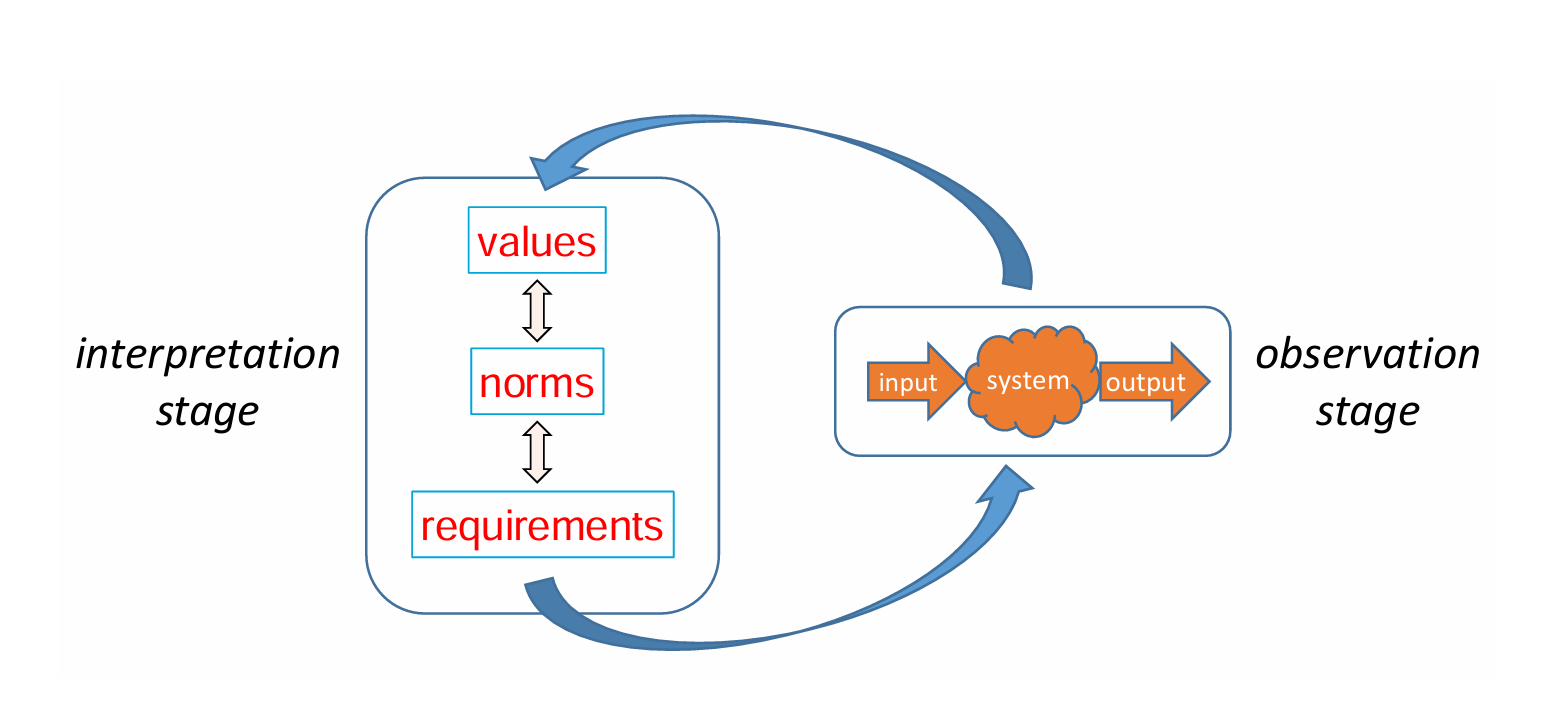
\includegraphics[width=0.8\textwidth]{images/GlassBox.png}
% 	\caption{The two stages of the Glass-Box Approach: an Interpretation stage, where values are translated into design requirements, and an Observation stage, where we can observe and qualify the behaviour of the system} % de caption komt verbatim uit de oorspronkelijke paper
% 	\label{fig:glassbox}
% \end{figure}

\subsection{Sociotechnical Layer}
At the sociotechnical layer, the previously described opacity intersects with documented human-factors. \citet{parasuraman2010complacency} describe automation complacency as the disengagement which occurs in reliable automated systems, leading to insufficient monitoring. \citet{aimag.v40i1.2848} extend this to military context, citing the 2003 friendly fire of a British Tornado. Where a human operator was nominally in the loop, yet due to the engagement tempo the decision effectively being delegated to the system.

\citet{mhcof} define two conditions for genuine moral responsibility: adequate information and meaningful freedom of action. As identified in the previous section, operators which receive recommendations without reasoning chains and the reported twenty second per target window \citep{abraham_2024} make this practically infeasible. \citet{miller2018explanationartificialintelligenceinsights} adds to this that explanation is a fundamental social process between explainer and explainee, aided by knowledge and context. When all of these are not properly integrated, the operators approval carries a reduced moral and legal weight.

Former IDF intelligence officers describe this as a rubber-stamp process \citep{abraham_2024, kozlovski2024algorithms}. Choices which normally take extended deliberation over distinction, proportionality and precaution are in practice a single confirmation button.

\subsection{Governance Layer}
The structural failures in the other layers become institutional ones. \citet{unesco2021recommendation}, the first global standard on AI ethics, adopted by all 193 UNESCO member states, establishes human oversight as a non-delegable principle, any life and or death decision cannot be ceded to AI systems. They also introduce the Ethical Impact Assessment as a mechanism for assessing high-risk technologies. Of which UNESCO calls for transparency about whether such assessments have taken place and what oversight structures govern an AI system, even when technical details remain classified. There currently is no public known accountability framework for Habsora.

\citet{aimag.v40i1.2848}'s accountability gap sharpens this further, responsibility for each strike is distributed across personnel: model developers, training data suppliers, analysts and operators approving them. This diffusion makes that no single actor can be held responsible, a problem which the literature identifies as one of the central governance challenges. \citet{friedman2013vsd}'s Value Sensitive Design framework adds to this by specifying indirect stakeholders, those affected without directly using the system, such as civilians in the target environment. Additionaly, as assessed by the IDF, the complementary 'Lavender'-system (individual targeting system) has an approximate 10\% error rate which raises the question whether all feasible precautions to protect civilians are taken.


\newpage


% \subsubsubsection{\textbf{Failures}}
% Deep neural network which inherently is opaque, can't see reasoning.
% No evidence that they have XAI tools like SHAP or Grad-CAM which can help.
% \subsubsubsection{\textbf{Evidence}}
% Commanders report no visibility into which signals shape the decision.
% The IHL assessment requires to know \textit{why} something was selected, else there would be no legal grounds.
% \subsubsubsection{\textbf{Impact}}
% \citet{khan2021ethicsaisystematicliterature} Maps into this with: \textbf{P-01} transparency, \textbf{P-03} accountability, \textbf{CH-06} no technical understanding \& \textbf{CH09} no legal framework.
% Commanders cannot give real judgement as they cannot understand it with e.g. XAI.

% \subsection{Sociotechnical Layer}
% \subsubsubsection{\textbf{Failures}}
% Automation bias, people trust AI outputs too much, gradual stamp approvement. Also with the short time window this effect is amplified.
% \citet{mhcof} argue that you need two conditions to responsibility: adequate information and meaningful freedom of action. With the previous sentence discarding both. 
% \citet{miller2018explanationartificialintelligenceinsights} shows that from social science we have an explainer and explainee. Without showing what went into a decision people can't make real decisions when they only get a recommendation. 
% Combined with the volume it makes it fully impossible, thus no moral or legal weight.
% \subsubsubsection{\textbf{Evidence}}
% Former IDF commands mention rubber stamping/click approve.
% \subsubsubsection{\textbf{Impact}}
% IDF commanders, get 'responsibility' for something they can't even evaluate + civilian targetet by the system. Which 'normally' takes a long time of real oversight and weighings, and are now reduced to a button press.

% \subsection{Governance Layer}
% \subsubsubsection{\textbf{Failures}}
% UNESCO says it's not legal to delegate life-or-death choices to an AI system. 
% \citet{aimag.v40i1.2848}'s accountability cap is applicable. The responsibilities go: developers -> habsora algorithm -> IDF officer with recommendations -> approving commander. Thus spreading 'responsibility' when someone dies. 
% No ethical/stakeholder impact assessment, such as VSD
% \subsubsubsection{\textbf{Evidence}}
% 10\% error tolerance in recommendations. 
% Civilians are stakeholders, and certainly not consulted. 
% \subsubsubsection{\textbf{Impact}}
% World wide IHL